\section{Event Tracing for Windows (ETW)}

\subsection{Introduction}


According to Microsoft, \href{https://web.archive.org/web/20200725154736/https://docs.microsoft.com/en-us/archive/blogs/ntdebugging/part-1-etw-introduction-and-overview}{Event Tracing For Windows (ETW)} is a general-purpose, high-speed tracing facility provided by the operating system. Using a buffering and logging mechanism implemented in the kernel, ETW provides a tracing mechanism for events raised by both user-mode applications and kernel-mode device drivers

\subsection{Architecture and components}

\begin{figure}[!ht]
    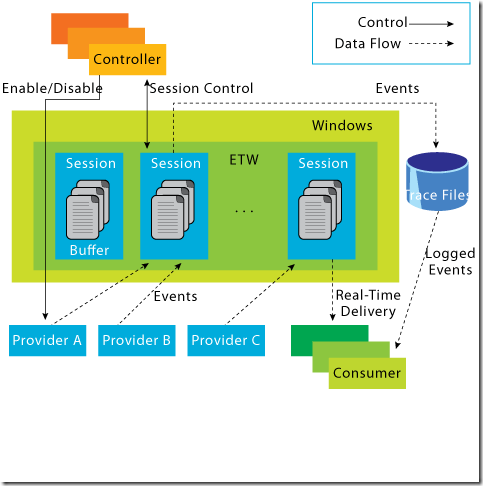
\includegraphics[width=\linewidth]{windows_knowledge/eventlog/images/etw-archi.png}
    \caption{ETW Architecture and Components}
    \label{fig:etw-archi}
\end{figure}


\subsubsection{Controllers}
\begin{itemize}
    \item Assumes control over all aspects related to ETW operations. It encompasses functionalities such as initiating and terminating trace sessions, as well as enabling or disabling providers within a particular trace. 
    \item Trace sessions can establish subscriptions to one or multiple providers, thereby granting the providers the ability to commence logging operations.
\end{itemize}

\verb+logman.exe+ is the builtin controller.

\subsubsection{Providers}

\begin{itemize}
    \item Providers play a pivotal role in generating events and writing them to the designated ETW sessions. 
    \item Applications have the ability to register ETW providers, enabling them to generate and transmit numerous events.
\end{itemize}

There are four distinct types of providers utilized within ETW:
\begin{itemize}
    \item MOF Providers: based on Managed Object Format (MOF) and are capable of generating events according to predefined MOF schemas. They offer a flexible approach to event generation and are widely used in various scenarios.
    \item WPP (Windows Software Trace Preprocessor) Providers: leverage specialized macros and annotations within the application's source code to generate events. This type of provider is often utilized for low-level kernel-mode tracing and debugging purposes.
    \item Manifest-based Providers:  represent a more contemporary form of providers within ETW. They rely on XML manifest files that define the structure and characteristics of events. This approach offers enhanced flexibility and ease of management, allowing for dynamic event generation and customization.
    \item TraceLogging Providers:  offer a simplified and efficient approach to event generation. They leverage the TraceLogging API, introduced in recent Windows versions, which streamlines the process of event generation with minimal code overhead.
\end{itemize}

Some event providers generate a significant volume of events, which can potentially overwhelm the system resources if they are constantly active. As a result, to prevent unnecessary resource consumption, these providers are typically disabled by default and are only enabled when a tracing session specifically requests their activation.

ETW can be extended through custom event providers.

{\bf Restricted Providers}:
These providers (\verb+Microsoft-Windows-Threat-Intelligence+ for example) offer valuable telemetry but are only accessible to processes that carry the requisite permissions (rotected Process Light (PPL)). This exclusivity is designed to ensure that sensitive system data remains shielded from potential threats.

\href{https://posts.specterops.io/uncovering-windows-events-b4b9db7eac54}{Workarounds to access the Microsoft-Windows-Threat-Intelligence provider.}

{\bf Useful Providers}:
\begin{itemize}
    \item \verb+icrosoft-Windows-Kernel-Process+:
    \item \verb+Microsoft-Windows-Kernel-File+:
    \item \verb+Microsoft-Windows-Kernel-Network+:
    \item \verb+Microsoft-Windows-Kernel-Registry+:
    \item \verb+Microsoft-Windows-SMBClient/SMBServer+:
    \item \verb+Microsoft-Windows-DotNETRuntime+:
    \item \verb+OpenSSH+:
    \item \verb+WinRM+:
    \item \verb+Microsoft-Windows-TerminalServices-LocalSessionManager+:
\end{itemize}

\subsubsection{Consumers}
\begin{itemize}
    \item  Consumers subscribe to specific events of interest and receive those events for further processing or analysis.
    \item By default, the events are typically directed to an .ETL (Event Trace Log) file for handling. However, an alternative consumer scenario involves leveraging the capabilities of the Windows API to process and consume the events.
\end{itemize}

\subsubsection{Channels}

To facilitate efficient event collection and consumption, ETW relies on event channels. Event channels act as logical containers for organizing and filtering events based on their characteristics and importance. ETW supports multiple channels, each with its own defined purpose and audience. Event consumers can selectively subscribe to specific channels to receive relevant events for their respective use cases.

\href{https://medium.com/threat-hunters-forge/threat-hunting-with-etw-events-and-helk-part-1-installing-silketw-6eb74815e4a0}{Only ETW provider events that have a Channel property applied to them can be consumed by the event log}

\subsubsection{ETL files}

ETW provides specialized support for writing events to disk through the use of event trace log files, commonly referred to as "ETL files." These files serve as durable storage for events, enabling offline analysis, long-term archiving, and forensic investigations. ETW allows for seamless rotation and management of ETL files to ensure efficient storage utilization.



\subsection{Logman (cmdline) /proformance monitor (gui)}


\begin{verbatim}
# list tracing sessions
logman.exe query -ets

# get infos on a tracing session
logman.exe query <session_name> -ets

# list providers
logman.exe query providers

# get infos on a provider
logman.exe query providers <provider_name>
\end{verbatim}


\subsection{Tools}

\subsubsection{SilkETW}

\href{https://github.com/mandiant/SilkETW}{SilkETW}

\begin{verbatim}
SilkETW.exe -t user -pn Microsoft-Windows-DotNETRuntime -uk 0x2038 -ot file -p C:\tools\etw.json
\end{verbatim}


\subsection{Links}

\begin{itemize}
    \item \href{https://nasbench.medium.com/a-primer-on-event-tracing-for-windows-etw-997725c082bf}{https://nasbench.medium.com/a-primer-on-event-tracing-for-windows-etw-997725c082bf}
    \item \href{https://bmcder.com/blog/a-begginers-all-inclusive-guide-to-etw}{https://bmcder.com/blog/a-begginers-all-inclusive-guide-to-etw}
\end{itemize}